\documentclass[letterpaper]{article} % DO NOT CHANGE THIS
\usepackage[submission]{aaai2027}  % DO NOT CHANGE THIS
% The serif, sans-serif, and monospaced fonts are loaded automatically by
% aaai2027.sty (newtxtext, helvet, courier). DO NOT add \usepackage{times},
% \usepackage{helvet}, \usepackage{courier}, or any other font package.
\usepackage[hyphens]{url}  % DO NOT CHANGE THIS
\usepackage{graphicx} % DO NOT CHANGE THIS
\urlstyle{rm} % DO NOT CHANGE THIS
\def\UrlFont{\rm}  % DO NOT CHANGE THIS
\usepackage{natbib}  % DO NOT CHANGE THIS AND DO NOT ADD ANY OPTIONS TO IT
\usepackage{caption} % DO NOT CHANGE THIS AND DO NOT ADD ANY OPTIONS TO IT
\usepackage{amsmath,amssymb}
\frenchspacing  % DO NOT CHANGE THIS
%
% These are recommended to typeset algorithms but not required. See the subsubsection on algorithms. Remove them if you don't have algorithms in your paper.
\usepackage{algorithm}
\usepackage{algorithmic}

%
% These are recommended to typeset listings but not required. See the subsubsection on listing. Remove this block if you don't have listings in your paper.
\usepackage{newfloat}
\usepackage{listings}
\DeclareCaptionStyle{ruled}{labelfont=normalfont,labelsep=colon,strut=off} % DO NOT CHANGE THIS
\lstset{%
	basicstyle={\footnotesize\ttfamily},% footnotesize acceptable for monospace
	numbers=left,numberstyle=\footnotesize,xleftmargin=2em,% show line numbers, remove this entire line if you don't want the numbers.
	aboveskip=0pt,belowskip=0pt,%
	showstringspaces=false,tabsize=2,breaklines=true}
\floatstyle{ruled}
\newfloat{listing}{tb}{lst}{}
\floatname{listing}{Listing}

%
% Recommended for better-looking tables
\usepackage{booktabs}

%
% Keep the \pdfinfo as shown here. There's no need
% for you to add the /Title and /Author tags.
\pdfinfo{
/TemplateVersion (2027.1)
}

% DISALLOWED PACKAGES
% \usepackage{authblk} -- This package is specifically forbidden
% \usepackage{balance} -- This package is specifically forbidden
% \usepackage{CJK} -- This package is specifically forbidden
% \usepackage{float} -- This package is specifically forbidden
% \usepackage{flushend} -- This package is specifically forbidden
% \usepackage{fullpage} -- This package is specifically forbidden
% \usepackage{geometry} -- This package is specifically forbidden
% \usepackage{hyperref} -- This package is specifically forbidden
% \usepackage{navigator} -- This package is specifically forbidden
% (or any other package that embeds links such as navigator or hyperref)
% \usepackage{indentfirst} -- This package is specifically forbidden
% \usepackage{layout} -- This package is specifically forbidden
% \usepackage{multicol} -- This package is specifically forbidden
% \usepackage{nameref} -- This package is specifically forbidden
% \usepackage{savetrees} -- This package is specifically forbidden
% \usepackage{setspace} -- This package is specifically forbidden
% \usepackage{stfloats} -- This package is specifically forbidden
% \usepackage{tabu} -- This package is specifically forbidden
% \usepackage{titlesec} -- This package is specifically forbidden
% \usepackage{tocbibind} -- This package is specifically forbidden
% \usepackage{ulem} -- This package is specifically forbidden
% \usepackage{wrapfig} -- This package is specifically forbidden
% DISALLOWED COMMANDS
% \nocopyright -- Your paper will not be published if you use this command
% \addtolength -- This command may not be used
% \balance -- This command may not be used
% \baselinestretch -- Your paper will not be published if you use this command
% \clearpage -- No page breaks of any kind may be used for the final version of your paper
% \columnsep -- This command may not be used
% \newpage -- No page breaks of any kind may be used for the final version of your paper
% \pagebreak -- No page breaks of any kind may be used for the final version of your paper
% \pagestyle -- This command may not be used
% \tiny -- This is not an acceptable font size.
% \vspace{- -- No negative value may be used in proximity of a caption, figure, table, section, subsection, subsubsection, or reference
% \vskip{- -- No negative value may be used to alter spacing above or below a caption, figure, table, section, subsection, subsubsection, or reference

\setcounter{secnumdepth}{0} %May be changed to 1 or 2 if section numbers are desired.

% The file aaai2027.sty is the style file for AAAI Press
% proceedings, working notes, and technical reports.
%

% Title

% Your title must be in mixed case, not sentence case.
% That means all verbs (including short verbs like be, is, using,and go),
% nouns, adverbs, adjectives should be capitalized, including both words in hyphenated terms, while
% articles, conjunctions, and prepositions are lower case unless they
% directly follow a colon or long dash
%\title{AAAI Press Anonymous Submission\\Instructions for Authors Using \LaTeX{}}
\title{MM-Mixer: A Simple Yet Strong Baseline for Multimodal Emotion Recognition in Conversations}
\author{
    %Authors
    % All authors must be in the same font size and format.
    Written by AAAI Press Staff\textsuperscript{\rm 1}\thanks{With help from the AAAI Publications Committee.}\\
    AAAI Style Contributions by Peter Patel Schneider,
    Sunil Issar,\\
    J. Scott Penberthy,
    George Ferguson,
    Hans Guesgen,
    Francisco Cruz\equalcontrib\corresponding,
    Marc Pujol-Gonzalez\equalcontrib\corresponding
}
\affiliations{
    %Afiliations
    \textsuperscript{\rm 1}Association for the Advancement of Artificial Intelligence\\
    % If you have multiple authors and multiple affiliations
    % use superscripts in text and roman font to identify them.
    % For example,

    % Sunil Issar\textsuperscript{\rm 2},
    % J. Scott Penberthy\textsuperscript{\rm 3},
    % George Ferguson\textsuperscript{\rm 4}\corresponding,
    % Hans Guesgen\textsuperscript{\rm 5}
    % Note that the comma should be placed after the superscript

    1101 Pennsylvania Ave, NW Suite 300\\
    Washington, DC 20004 USA\\
    % email address must be in roman text type, not monospace or sans serif
    proceedings-questions@aaai.org
%
% See more examples next
}

%Example, Single Author, ->> remove \iffalse,\fi and place them surrounding AAAI title to use it
\iffalse
\title{My Publication Title --- Single Author}
\author {
    Author Name
}
\affiliations{
    Affiliation\\
    Affiliation Line 2\\
    name@example.com
}
\fi

\iffalse
%Example, Multiple Authors, ->> remove \iffalse,\fi and place them surrounding AAAI title to use it
\title{My Publication Title --- Multiple Authors}
\author {
    % Authors
    First Author Name\textsuperscript{\rm 1,\rm 2}\equalcontrib,
    Second Author Name\textsuperscript{\rm 2}\equalcontrib,
    Third Author Name\textsuperscript{\rm 1}\corresponding
}
\affiliations {
    % Affiliations
    \textsuperscript{\rm 1}Affiliation 1\\
    \textsuperscript{\rm 2}Affiliation 2\\
    firstAuthor@affiliation1.com, secondAuthor@affilation2.com, thirdAuthor@affiliation1.com
}
\fi


\begin{document}

\maketitle

\begin{abstract}
Multimodal Emotion Recognition in Conversation (MERC) aims to identify utterance-level emotions from the text, audio, and visual signals within a dialogue.
%textual, acoustic, and visual cues. 
Existing methods fuse unimodal representations and perform cross-modal interaction from a unified modality perspective, ignoring the utilization of complementary cross-modal interaction from different perspectives, such as the sequence dimension and the hidden feature dimension. Feature utilization from multiple perspectives can help the model capture sentiment cues from different modality signals more accurately.
%without explicitly separating axis-specific processing from complementary pairwise interactions. 
To address this issue, we propose a simple yet strong MERC framework named \textbf{MM-Mixer} to mine and model sentiment cues by performing cross-modal interaction and fusion from multiple perspectives. Specifically, the Adaptive Gating module is first deployed to extract modality-specific cues for subsequent modality-centric cross-modal alignment, which reduces irrelevant information before multimodal fusion. To extract multimodal sentiment cues from multiple perspectives, an Axis-wise Multimodal Mixer is proposed to perform cross-modal interaction along the latent sequence dimension, modality dimension, and hidden feature dimension in sequence. Finally, a simple fusion module enhanced with Explicit Pairwise Interaction Residual Correction is introduced to fuse all different modality features into a compact yet discriminative multimodal representation for emotion recognition. Extensive experiments on the IEMOCAP and MELD datasets show that our MM-Mixer consistently outperforms baselines in accuracy and weighted F1-score.

%Adaptive gating first filters modality-specific cues and forms a shared context for directional cross-modal refinement, reducing irrelevant information before deeper fusion. The Axis-wise Multimodal Mixer then processes the latent-subspace, modality, and channel axes separately, allowing within-modality organization, cross-modal exchange, and channel transformation to be handled by dedicated operations. The Explicit Pairwise Interaction Residual complements the main fusion pathway by capturing low-rank multiplicative dependencies across modality pairs and injecting them as residual corrections. Experiments on IEMOCAP and MELD under a unified history-only protocol show that MM-Mixer consistently outperforms representative causal baselines in weighted F1-score and accuracy

\end{abstract}

% Uncomment the following to link to your code, datasets, an extended version or similar.
% You must keep this block between (not within) the abstract and the main body of the paper.
% Make sure that you do not de-anonymize yourself with these links.
% \begin{links}
%     \link{Code}{https://aaai.org/example/code}
%     \link{Datasets}{https://aaai.org/example/datasets}
%     \link{Extended version}{https://aaai.org/example/extended-version}
% \end{links}
\section{Introduction}

Multimodal Emotion Recognition in Conversation (MERC) aims to identify the emotion expressed by each utterance in a dialogue by integrating textual, acoustic, and visual signals. Early ERC studies mainly focused on text-based conversational context and speaker dependencies through recurrent state tracking and graph-based reasoning~\cite{dialoguernn,dialoguegcn}. With the increasing availability of multimodal conversational data, subsequent MERC methods have incorporated acoustic and visual signals through multimodal graph learning~\cite{mmgcn}, cross-modal attention~\cite{dialoguetrm}, and more expressive fusion mechanisms~\cite{sdt,css}. These approaches have substantially advanced multimodal representation learning for MERC by enabling information exchange among heterogeneous modality streams.

Despite this progress, many existing MERC frameworks still treat each utterance-level modality-specific representation as a holistic interaction unit during multimodal fusion. Although such representations may contain rich affective information, interacting only at this granularity provides limited ability to mine the emotion cues distributed within them. Subtle but valuable cues may be obscured by dominant features, while complementary evidence distributed across textual, acoustic, and visual signals may be diluted by unified fusion operators. Consequently, the resulting multimodal representation may be insufficiently sensitive to subtle emotional expressions.

To address this limitation, we propose MM-Mixer, a simple yet strong framework for multimodal interaction. MM-Mixer first applies an Adaptive Gating module to filter modality-specific cues and construct a shared context for modality-centric cross-modal alignment. After the modality-centric cross-modal alignment, the core Axis-wise Multimodal Mixer is deployed to transform each utterance-level modality-specific representation into a fixed-length latent sequence and separately processes it along with the latent sequence, modality, and hidden-feature dimensions.
Here, the latent sequence comprises learned elements generated within each modality rather than temporally ordered conversational utterances. The latent-sequence-dimension mixing captures dependencies among latent elements. The modality-dimension mixing exchanges information among textual, acoustic, and visual streams. The hidden-feature-dimension mixing refines the internal
representation of each element. To obtain a compact yet discriminative multimodal representation for emotion recognition, a simple fusion module enhanced with Explicit Pairwise Interaction Residual Correction is introduced to fuse all different modality
features in a dual path. One main path is a simple fusion pathway to fuse all different modality
features in a unified way, while the residual path captures pairwise dependencies across modalities and injects them into the fused representation from the main path as a residual correction.
%To complement this axis-wise main pathway, an Explicit Pairwise Interaction Residual captures low-rank multiplicative dependencies across modality pairs and injects them into the fused representation as a residual correction.

Extensive experiments on popular MERC benchmarks, IEMOCAP~\cite{iemocap} and MELD~\cite{meld}, under a unified history-only protocol, where future conversational information is excluded during prediction, show that MM-Mixer achieves impressive performance in accuracy and weighted F1-score against representative baselines. Ablation studies further examine the effects of the Adaptive Gating module, Axis-wise Multimodal Mixer module, and fusion module enhanced with Explicit Pairwise Interaction Residual Correction.

%We evaluate MM-Mixer on IEMOCAP~\cite{iemocap} and MELD~\cite{meld} under a unified history-only protocol, where future conversational information is excluded during prediction. Experimental results show that MM-Mixer achieves competitive performance in accuracy and weighted F1-score against representative causal baselines. Controlled experiments further examine the effects of the Adaptive Gating module, Axis-wise Multimodal Mixer module, and explicit pairwise residual fusion module.

Our main contributions are summarized as follows:
\begin{itemize}
\item We propose MM-Mixer, a simple yet strong MERC framework that models multimodal emotion cues through progressive modality refinement and multi-dimensional interaction.
\item We introduce an Axis-wise Multimodal Mixer to extract multimodal sentiment cues from multiple perspectives by performing multi-dimensional feature interaction along the latent-sequence, modality, and hidden-feature dimensions.
\item We develop an Explicit Pairwise Interaction Residual Correction that captures pairwise dependencies across modalities and incorporates them as residual corrections to the main fused representation. 

\item Extensive experiments on popular MERC benchmarks, IEMOCAP and MELD, under a unified history-only protocol show that  MM-Mixer achieves impressive performance in accuracy and weighted F1-score against representative baselines.
\end{itemize}
\section{Related Work}

\noindent\textbf{Context Modeling in ERC.}
Conversational context provides important evidence for interpreting an utterance whose emotion cannot be determined in isolation. Sequence-based methods model this evidence by tracking dialogue and speaker states. For example, DialogueRNN~\cite{dialoguernn} maintains speaker-specific states together with a global dialogue state. Graph-based methods instead represent utterances as nodes and propagate information through speaker-dependent relations, as in DialogueGCN~\cite{dialoguegcn}. DAG-ERC~\cite{dagerc} further organizes information flow with a directed acyclic graph that combines local and long-range context. These methods mainly differ in how information is propagated across utterances and speakers. More recently, PRC-Emo~\cite{prcemo} combines emotion-sensitive prompting, demonstration retrieval, and a curriculum based on weighted emotion shifts between same- and different-speaker utterances to model explicit and implicit contextual cues.

MM-Mixer does not introduce a new dialogue topology and focuses on multimodal interaction after the causal textual context has been encoded.

\noindent\textbf{Multimodal Interaction and Fusion.}
MERC methods must combine heterogeneous textual, acoustic, and visual signals while retaining information specific to each modality. MMGCN~\cite{mmgcn} constructs a multimodal graph to model cross-modal and speaker-dependent relations, while MMDAG~\cite{mmdag} extends directed acyclic context modeling to multimodal inputs. Transformer-based approaches use intra- and inter-modal attention for direct information exchange. DialogueTRM~\cite{dialoguetrm} follows this strategy to model multimodal emotional dynamics, and SDT~\cite{sdt} combines intra- and inter-modal Transformers with gated fusion and unimodal self-distillation. Other methods introduce task-specific interaction structures. ECERC~\cite{ecerc} separates target-utterance evidence from contextual causes, whereas GS-MCC~\cite{gsmcc} models multimodal conversations through graph-spectral operators. Recent work has also moved toward asymmetric or component-aware fusion. EMART~\cite{emart} treats text as the primary information source and audio as a complementary signal, coupling modality-aware fusion with an emotion-wheel-guided supervised contrastive objective. DnR~\cite{dnr} explicitly decomposes multimodal representations into unique, pairwise redundant, and synergistic components before applying component-specific refinement. Together, these methods organize multimodal reasoning through graph propagation, attention-based exchange, or task-specific interaction structures.

Compared with these methods, MM-Mixer organizes multimodal interaction according to the internal structure of the utterance-level representation. It assigns dedicated transformations to the learned-sequence, modality, and hidden-feature axes, enabling structured information exchange with a lightweight mixer architecture.

\noindent\textbf{Axis-Factorized and Multiplicative Interaction.}
Axis-factorized networks assign different transformations to different dimensions of a representation. MLP-Mixer~\cite{mlpmixer} separates token mixing from channel mixing, demonstrating that interactions along these two axes can be modeled by dedicated MLPs. Multiplicative fusion provides another way to expose cross-modal dependencies. Factorized bilinear pooling and low-rank multimodal fusion approximate tensor interactions without constructing a full outer-product tensor~\cite{mfb,lmf}. In MERC, CSS~\cite{css} uses low-rank polynomial fusion as its main multimodal fusion operator and coordinates multiple objectives through Pareto gradient modulation.





\section{Methodology}

\begin{figure*}[t]
\centering
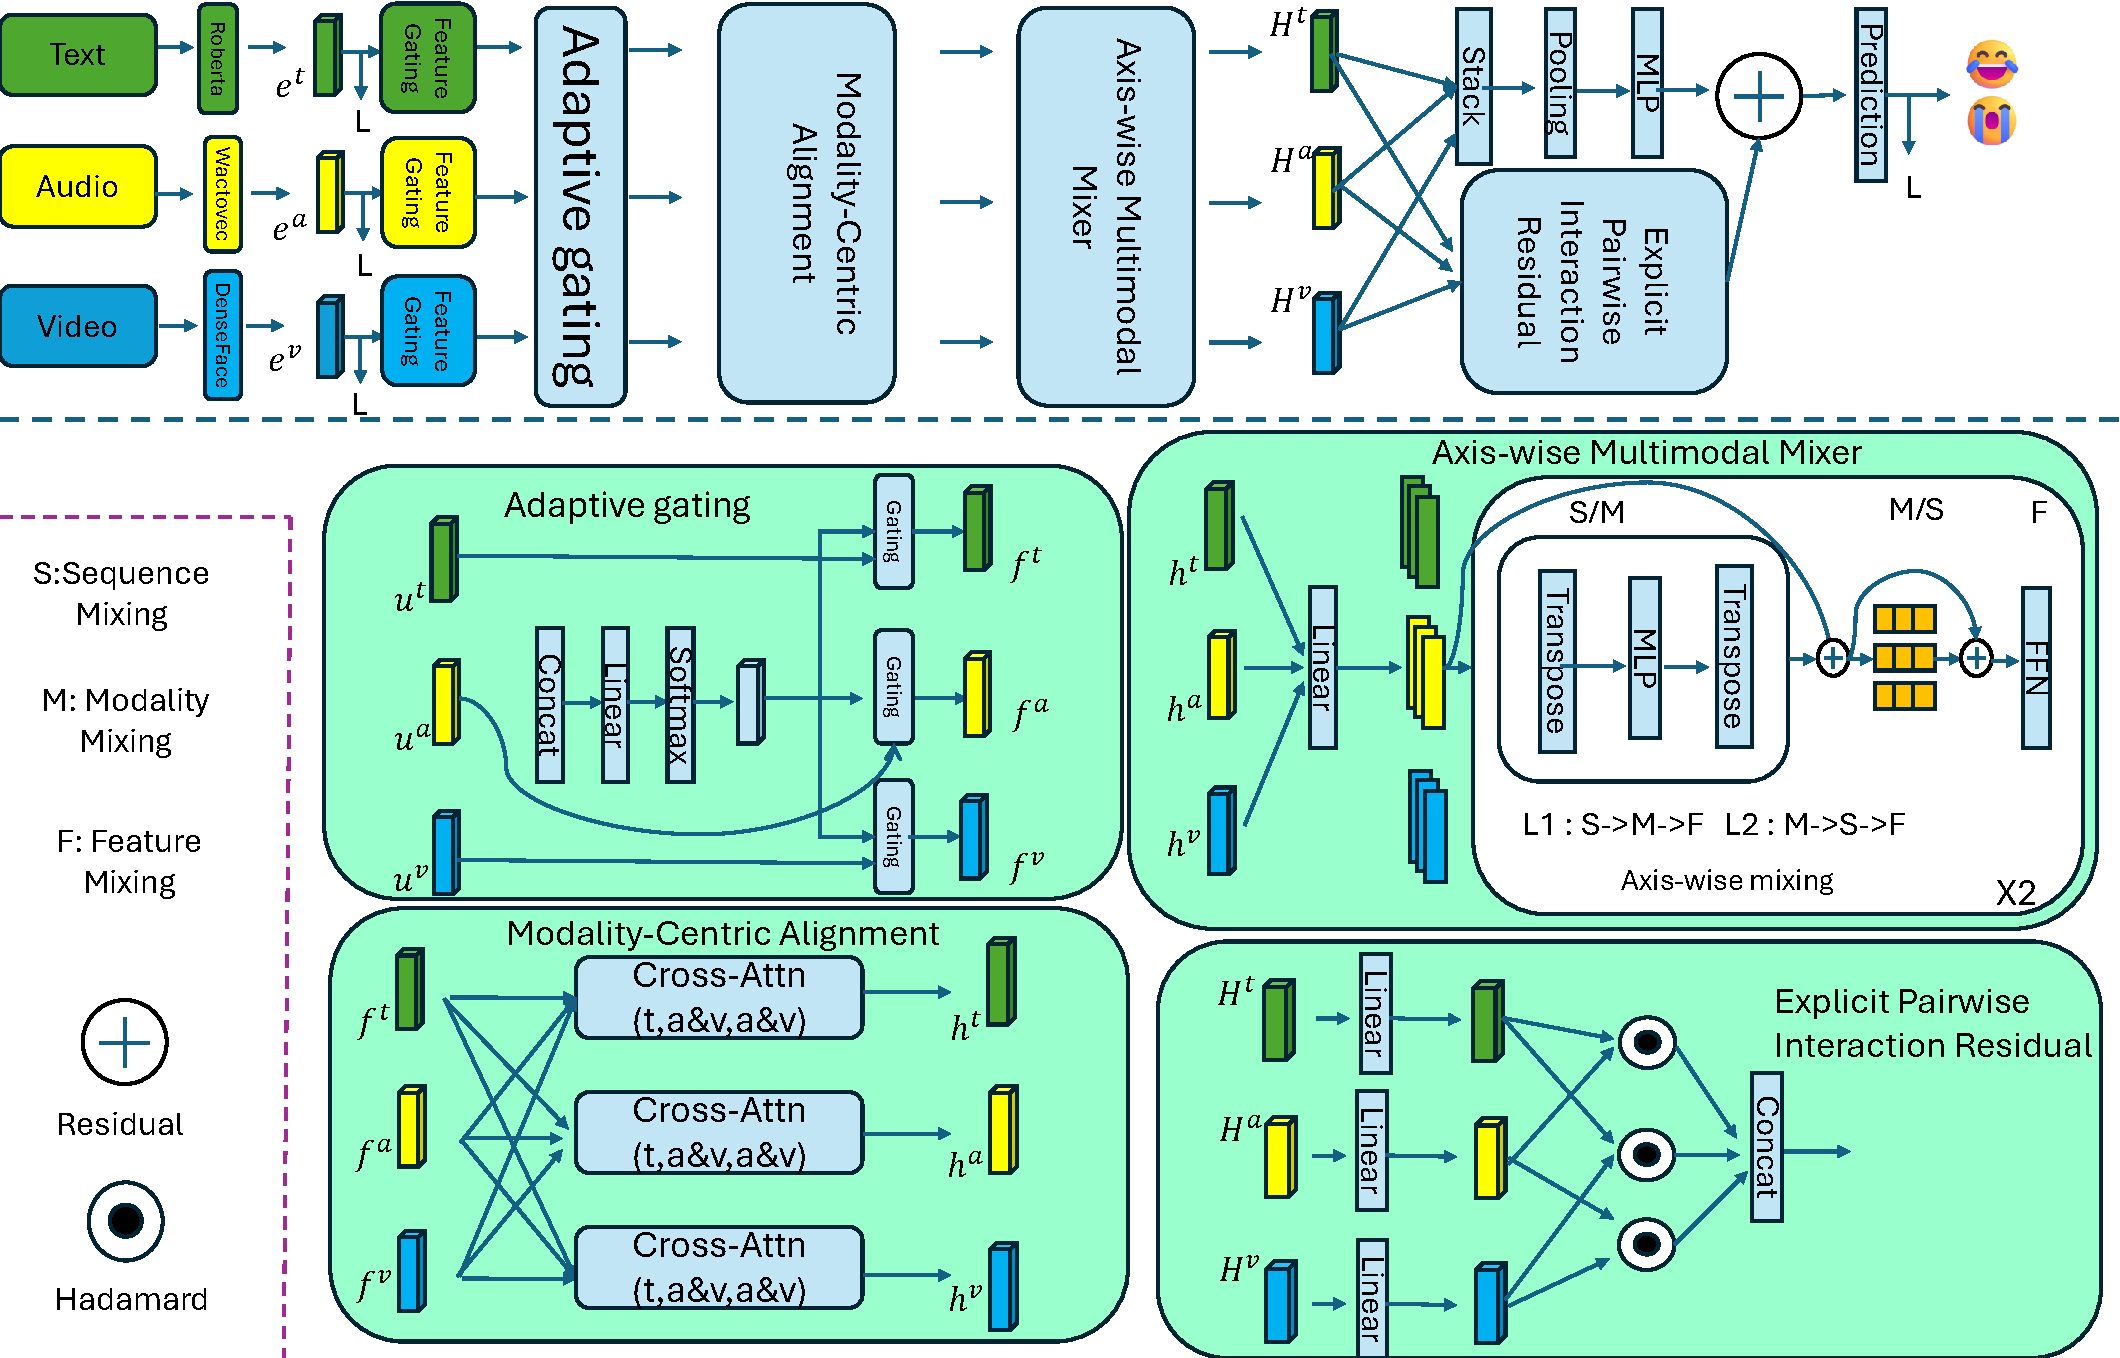
\includegraphics[width=0.99\textwidth]{MM-Mixer.pdf}
\caption{Overview of MM-Mixer. Pre-extracted textual, acoustic, and
visual features are projected and gated before adaptive refinement and
modality-centric cross-modal alignment. Two alternating axis-wise mixer
blocks organize the resulting representations along the latent-sequence,
modality, and feature dimensions. Query-based integration forms the
main prediction pathway, while explicit low-rank pairwise interactions
provide a residual correction. Layer normalization and internal
residual connections are omitted for clarity.}
\label{fig:mm_mixer}
\end{figure*}

\subsection{MM-Mixer Overview}
Given a dialogue $\{u_t\}_{t=1}^{N}$ containing $N$ utterances, MERC
aims to predict an emotion label $y_t\in\{1,\ldots,C\}$ for each
utterance $u_t$. The model input contains a textual feature
$\mathbf{x}^{T}_{t}\in\mathbb{R}^{d_T}$, an acoustic feature
$\mathbf{x}^{A}_{t}\in\mathbb{R}^{d_A}$, and a visual feature
$\mathbf{x}^{V}_{t}\in\mathbb{R}^{d_V}$. The superscripts $T$, $A$,
and $V$ identify the textual, acoustic, and visual modalities,
respectively. The textual feature represents the target utterance
together with its preceding dialogue context, whereas the acoustic and
visual features describe the target utterance. All inputs exclude
utterances after $u_t$. MM-Mixer learns a mapping $f_{\theta}$ from the
three modality features to the emotion space and selects the class with
the highest predicted probability:
\begin{equation}
\widehat{y}_{t}
=\underset{c\in\{1,\ldots,C\}}{\operatorname{argmax}}\,
f_{\theta}\!\left(
\mathbf{x}^{T}_{t},\mathbf{x}^{A}_{t},\mathbf{x}^{V}_{t}
\right)_{c}
\label{eq:task_definition}
\end{equation}
where $f_{\theta}$ denotes the model parameterized by $\theta$, and
$\widehat{y}_{t}$ is the predicted emotion label of $u_t$.
For clarity, the utterance index $t$ is omitted below.

As illustrated in Figure~\ref{fig:mm_mixer}, MM-Mixer first employs pre-trained modality-specific encoders to extract utterance-level unimodal features and projects them
into a common feature space. Modality-specific feature gates suppress
irrelevant channels. Adaptive Gating (AG) then constructs a shared
multimodal reference and uses it to calibrate each modality, after which
Modality-centric Cross-modal Alignment (MCA) uses each modality to query
complementary information from the other two modalities. The aligned
representations are then organized along the learned-sequence, modality,
and hidden-feature axes by the Axis-wise Multimodal Mixer (AMM).
Finally, query-based integration forms the main fusion pathway, while
the Explicit Pairwise Interaction Residual Correction (EPIRC) branch provides an
additive low-rank multiplicative correction. The fused prediction and
three unimodal predictions are jointly optimized during training.

%operates on pre-extracted utterance-level features from the textual, acoustic, and visual streams.  
%The modality set is $\mathcal{M}=\{T,A,V\}$, and $D$ denotes the common feature width.
%For $m\in\mathcal{M}$, $\mathbf{x}^{m}\in\mathbb{R}^{d_m}$ denotes the pre-extracted input feature of modality $m$.

%Throughout this section, $\mathbf{W}$ and $\mathbf{b}$ are learned parameters; $\operatorname{LN}$, $\sigma$, and $\odot$ denote layer normalization, the sigmoid function, and element-wise multiplication, respectively. A semicolon inside brackets denotes concatenation.



\subsection{Unimodal Feature Extraction}
MM-Mixer first deploys pre-trained modality-specific encoders to extract utterance-level unimodal features $\mathbf{x}^{T}$, $\mathbf{x}^{A}$, and $\mathbf{x}^{V}$. Since the input modalities have different feature dimensions and feature
distributions, each modality is projected into a common feature space to reduce their heterogeneity, followed by filtering irrelevant information with a feature gating as follows:
\begin{equation}
\begin{aligned}
\mathbf{e}^{m}
&=\operatorname{Dropout}\!\left(
  \operatorname{GELU}\!\left(
  \operatorname{LN}(\mathbf{W}_{p}^{m}\mathbf{x}^{m}
  +\mathbf{b}_{p}^{m})\right)\right) \\
\mathbf{coff}^{m} &= \sigma\!\left(\mathbf{W}_{g2}^{m}
  \operatorname{ReLU}\!\left(
  \operatorname{LN}(\mathbf{W}_{g1}^{m}\mathbf{e}^{m}
  +\mathbf{b}_{g1}^{m})\right)+\mathbf{b}_{g2}^{m}\right) \\
\mathbf{u}^{m} & =\mathbf{e}^{m}\odot \mathbf{coff}^{m}
\end{aligned}
\label{eq:feature_gating}
\end{equation}
where $\mathbf{e}^{m}\in\mathbb{R}^{D}$ is the unimodal representation, $\mathbf{u}^{m}\in\mathbb{R}^{D}$ is its refined version, and $m\in M$, with $M=\{T,A,V\}$. $\mathbf{W}_{p}^{m}$, $\mathbf{W}_{g1}^{m}$ and $\mathbf{W}_{g2}^{m}$ are learnable weights. $\mathbf{b}_{p}^{m}$, $\mathbf{b}_{g1}^{m}$ and $\mathbf{b}_{g2}^{m}$ are learnable biases. $\operatorname{Dropout}$, $\operatorname{GELU}$, $\operatorname{ReLU}$, and $\operatorname{LN}$ denote the dropout, GELU activation, RELU activation, and layer normalization, respectively. $\sigma$ denotes the Sigmoid function. Here, it is used to suppress irrelevant channels while preserving one feature vector per modality.

%Here, $\mathbf{e}^{m}\in\mathbb{R}^{D}$ is the projected unimodal
%feature supplied to a modality-specific feature gate:
%\begin{equation}
%\mathbf{u}^{m}
%=\mathbf{e}^{m}\odot
%  \sigma\!\left(\mathbf{W}_{g2}^{m}
%  \operatorname{ReLU}\!\left(
%  \operatorname{LN}(\mathbf{W}_{g1}^{m}\mathbf{e}^{m}
%  +\mathbf{b}_{g1}^{m})\right)+\mathbf{b}_{g2}^{m}\right)
%\label{eq:feature_gating}
%\end{equation}
%Here, $\mathbf{u}^{m}\in\mathbb{R}^{D}$ is the gated feature. The sigmoid
%coefficients suppress unhelpful channels while preserving one vector
%per modality.

\subsection{Adaptive Gating}
Given the filtered unimodal features, the AG module constructs a shared multimodal
reference as follows:
\begin{equation}
\begin{aligned}
\boldsymbol{\alpha}
&=\operatorname{softmax}\!\left(
  \operatorname{MLP}([\mathbf{u}^{T};
  \mathbf{u}^{A};\mathbf{u}^{V}])\right)\\
\mathbf{c}
&=\sum_{m\in M}\alpha_m\mathbf{u}^{m}
\end{aligned}
\label{eq:adaptive_context}
\end{equation}
where $\boldsymbol{\alpha}\in\mathbb{R}^{3}$ contains the normalized modality
coefficients, and $\mathbf{c}\in\mathbb{R}^{D}$ is their weighted
multimodal reference. The shared reference then conditions a separate
channel gate to calibrate modality features for each modality:
\begin{equation}
\mathbf{f}^{m}
=\left[
  \sigma\!\left(\operatorname{MLP}_{c}^{m}
  ([\mathbf{u}^{m};\mathbf{c}])\right)+\epsilon_g
  \right]\odot\mathbf{u}^{m}
\label{eq:channel_calibration}
\end{equation}
Here, $\mathbf{f}^{m}\in\mathbb{R}^{D}$ is the calibrated modality
feature. The context-conditioned sigmoid coefficients perform channel
selection, while $\epsilon_g$ preserves a direct contribution from
$\mathbf{u}^{m}$.

\subsection{Modality-centric Cross-modal Alignment}

The MCA module comprises three directional cross-attention branches.
For each $m\in M$, one branch uses the calibrated feature of
modality $m$ as its query, while the other two modalities provide the
keys and values:
\begin{equation}
\begin{aligned}
\mathbf{K}^{m}=\mathbf{V}^{m}
&=\operatorname{Stack}\{\mathbf{f}^{n}
  \mid n\in M,\,n\neq m\}\\
\mathbf{h}^{m}
&=\operatorname{MHA}^{m}
  (\mathbf{f}^{m},\mathbf{K}^{m},\mathbf{V}^{m})
  +\epsilon_a\mathbf{f}^{m}
\end{aligned}
\label{eq:cross_modal_attention}
\end{equation}
Here, $\mathbf{K}^{m}$ and $\mathbf{V}^{m}\in\mathbb{R}^{2\times D}$
contain the two peer-modality vectors.
$\operatorname{MHA}^{m}$ is the multi-head attention layer for query modality
$m$, and $\epsilon_a$ controls the query residual. The output
$\mathbf{h}^{m}\in\mathbb{R}^{D}$ is the cross-modal aligned feature of
modality $m$. %the three outputs retain the fixed order $V,A,T$.

\subsection{Axis-wise Multimodal Mixer}
AMM aims to mine the sentiment cues along different dimensions from the cross-modal aligned feature $\mathbf{h}^{m}$, since the three axes of a multimodal representation have different meanings: learned elements within a modality, modality identity, and hidden feature channels. AMM processes these axes separately so that each operation has a defined input dimension and interaction scope.

%The three axes of a multimodal representation have different meanings: learned elements within a modality, modality identity, and hidden feature channels. 
%We process these axes separately so that each operation has a defined input dimension and interaction scope.


\noindent\textbf{Sequence construction.} For every modality, a shared linear map expands one $D$-dimensional vector $\mathbf{h}^{m}$ into a sequence of $S$ learned elements, and then these sequences are stacked as a complete multimodal tensor $\mathbf{Z}^{0}\in\mathbb{R}^{3\times S\times D}$:
\begin{equation}
\mathbf{Z}^{0} =\operatorname{Stack}_{m\in M}
  \left[
  \operatorname{reshape}_{S\times D}
  (\mathbf{W}_{s}\mathbf{h}^{m}+\mathbf{b}_{s})
  \right]
\label{eq:sequence_construction}
\end{equation}
%Here, $\mathbf{Z}^{0}\in\mathbb{R}^{3\times S\times D}$ is the complete multimodal tensor, and 
where the parameters $\mathbf{W}_{s}$ and $\mathbf{b}_{s}$ are shared by
$T$, $A$, and $V$, giving corresponding sequence coordinates a common
parameterization. The modality axis of $\mathbf{Z}^{0}$ follows the
fixed order $V,A,T$.

For the sake of consistency, the notation $[\cdot]_{m,s,d}$ denotes an
entry at modality $m$, learned-sequence element $s$, and feature channel
$d$ in the remaining part. 

\noindent\textbf{Axis-wise mixing.}
Each mixer block contains three pre-normalized residual operators. Let $\mathbf{Z}\in\mathbb{R}^{3\times S\times D}$ denote a generic input to an axis-mixing operator. Sequence mixing applies an MLP along the $S$ axis while holding the modality and feature indices fixed:
\begin{equation}
[\mathcal{S}(\mathbf{Z})]_{m,:,d}
=[\mathbf{Z}]_{m,:,d}
+\operatorname{MLP}_{S}
  \bigl([\operatorname{LN}_{S}(\mathbf{Z})]_{m,:,d}\bigr).
\label{eq:sequence_mixing}
\end{equation}
Here, $\operatorname{MLP}_{S}$ maps the sequence axis through a hidden
layer and returns an output of the same width.

Modality mixing instead holds $(s,d)$ fixed and transforms the
three-vector $\bigl[[\mathbf{Z}]_{V,s,d};
[\mathbf{Z}]_{A,s,d};[\mathbf{Z}]_{T,s,d}\bigr]$:
\begin{equation}
[\mathcal{M}(\mathbf{Z})]_{:,s,d}
=[\mathbf{Z}]_{:,s,d}
+\mathbf{W}_{r}
  [\operatorname{LN}_{M}(\mathbf{Z})]_{:,s,d}.
\label{eq:modality_mixing}
\end{equation}
The bias-free routing matrix
$\mathbf{W}_{r}\in\mathbb{R}^{3\times3}$ is shared across all sequence
coordinates and feature channels, providing a common cross-modal
transformation at every sequence-feature coordinate.

Feature mixing completes the block by applying a channel-wise MLP to every
modality--sequence pair:
\begin{equation}
[\mathcal{F}(\mathbf{Z})]_{m,s,:}
=[\mathbf{Z}]_{m,s,:}
+\operatorname{MLP}_{D}
  \bigl([\operatorname{LN}_{F}(\mathbf{Z})]_{m,s,:}\bigr).
\label{eq:feature_mixing}
\end{equation}
Here, $\mathcal{S}$, $\mathcal{M}$, and $\mathcal{F}$ denote sequence,
modality, and feature mixing, respectively.  The feature MLP follows
$D\!\rightarrow\!D_h\!\rightarrow\!D$ with GELU, where $D_h$ is its
hidden width.

We stack two mixer blocks with different operation orders:
\begin{equation}
\begin{aligned}
\mathbf{Z}^{1}
&=(\mathcal{F}^{1}\circ\mathcal{M}^{1}\circ\mathcal{S}^{1})
  (\mathbf{Z}^{0}) \\
\mathbf{Z}^{2}
&=(\mathcal{F}^{2}\circ\mathcal{S}^{2}\circ\mathcal{M}^{2})
  (\mathbf{Z}^{1}).
\end{aligned}
\label{eq:alternating_blocks}
\end{equation}
$\mathbf{Z}^{\ell}$ denotes the output tensor of mixer block $\ell$,
and the composition symbol $\circ$ is evaluated from right to left.
Therefore, the first mixer block organizes sequence elements before routing
across modalities, whereas the second routes modalities before sequence
refinement. Averaging over the sequence axis returns one vector per
modality:
\begin{equation}
\mathbf{H}^{m}=\frac{1}{S}\sum_{s=1}^{S}\mathbf{Z}^{2}_{m,s,:}
\label{eq:mixer_output}
\end{equation}
$\mathbf{H}^{m}\in\mathbb{R}^{D}$ is the mixer output for modality $m$.


\subsection{Multimodal Fusion with Explicit Pairwise Interaction Residual Correction}

Given the three modality representations produced by AMM, the
multimodal fusion contains a main fusion path and a parallel
residual path. The main path first stacks the mixer outputs along the
modality axis:
\begin{equation}
\mathbf{H}
=\operatorname{Stack}
  (\mathbf{H}^{V},
   \mathbf{H}^{A},
   \mathbf{H}^{T})
\label{eq:stacked_mixer_output}
\end{equation}
where $\mathbf{H}\in\mathbb{R}^{3\times D}$. Three learnable queries then aggregate the stacked modality representations via multi-head attention:
\begin{equation}
\mathbf{P}
=\operatorname{MHA}
  (\mathbf{Q}_{p},\mathbf{H},
   \mathbf{H})
\end{equation}
Here, $\mathbf{Q}_{p}\in\mathbb{R}^{3\times D}$ contains three learned
query vectors, and $\mathbf{P}$ contains their pooled outputs. The
outputs are flattened and integrated to form the main fused
representation $\mathbf{h}_{\mathrm{main}}\in\mathbb{R}^{D}$:
\begin{equation}
\mathbf{h}_{\mathrm{main}}
=\operatorname{MLP}_{\mathrm{int}}
  (\operatorname{vec}(\mathbf{P}))
\label{eq:main_fusion}
\end{equation}
where $\operatorname{vec}(\cdot)$ denotes the vectorization operation.
The integration MLP maps the flattened $3D$-dimensional representation
back to the common feature space.where $\operatorname{vec}(\cdot)$ denotes the vectorization operation.

Although the main fusion path adaptively aggregates the three modality
representations, it models their relations implicitly. To make the fused representation more discriminative, we introduce EPIRC as a parallel residual path that explicitly captures
multiplicative relations between modality pairs and uses them to correct the main fused representation. Each mixer output is first projected into a rank-$R$ space:
\begin{equation}
\mathbf{p}^{m}
=\mathbf{W}_{x}^{m}\mathbf{H}^{m}
+\mathbf{b}_{x}^{m}
\end{equation}
where $\mathbf{p}^{m}\in\mathbb{R}^{R}$ and $R$ is the interaction rank and $\mathbf{p}^{m}$ is the low-rank representation of modality $m$. Then, the explicit pairwise
interaction between two modalities is modeled as the product between two mixer outputs as follows:
\begin{equation}
\begin{aligned}
\mathbf{r}_{AV}&=\mathbf{p}^{A}\odot\mathbf{p}^{V}\\
\mathbf{r}_{TV}&=\mathbf{p}^{T}\odot\mathbf{p}^{V}\\
\mathbf{r}_{TA}&=\mathbf{p}^{T}\odot\mathbf{p}^{A}\\
\end{aligned}
\label{eq:pairwise_interact}
\end{equation}
where $\mathbf{r}_{AV}$, $\mathbf{r}_{TV}$, and $\mathbf{r}_{TA}$ encode the three modality-pair dependencies. After obtaining the interactions $\mathbf{r}_{AV}$, $\mathbf{r}_{TV}$, and $\mathbf{r}_{TA}$, the residual correction $\mathbf{r}\in\mathbb{R}^{D}$ can be computed as follows:
\begin{equation}
\begin{aligned}
\mathbf{r}_{\mathrm{cat}} &=[\mathbf{r}_{AV};\mathbf{r}_{TV};\mathbf{r}_{TA}]\\
\mathbf{r}&=\mathbf{W}_{o}\mathbf{r}_{\mathrm{cat}}
  +\mathbf{b}_{o}\in\mathbb{R}^{D}
\end{aligned}
\label{eq:pairwise_residual}
\end{equation}
where $;$ denotes the concatenation operation. $\mathbf{W}_{o}$ and $\mathbf{b}_{o}$ are initialized to zero, so this residual correction branch starts with a zero output and progressively learns a pairwise correction without perturbing the initial main fusion path.


%The three pairwise products are
%concatenated and projected to the common feature space:
%\begin{equation}
%\begin{aligned}
%&\mathbf{r}_{AV}=\mathbf{p}^{A}\odot\mathbf{p}^{V}\\
%&\mathbf{r}_{TV}=\mathbf{p}^{T}\odot\mathbf{p}^{V}\\
%&\mathbf{r}_{TA}=\mathbf{p}^{T}\odot\mathbf{p}^{A}\\
%&\mathbf{r}_{\mathrm{cat}}
%=[\mathbf{r}_{AV};\mathbf{r}_{TV};\mathbf{r}_{TA}]\\
%&\mathbf{r}=\mathbf{W}_{o}\mathbf{r}_{\mathrm{cat}}
%  +\mathbf{b}_{o}\in\mathbb{R}^{D}
%\end{aligned}
%\label{eq:pairwise_residual}
%\end{equation}
%$\mathbf{r}_{AV}$, $\mathbf{r}_{TV}$, and $\mathbf{r}_{TA}$ encode the
%three modality-pair products;
%$\mathbf{r}_{\mathrm{cat}}\in\mathbb{R}^{3R}$ is their concatenation;
%and $\mathbf{r}\in\mathbb{R}^{D}$ is the resulting residual correction.
%We initialize $\mathbf{W}_{o}$ and $\mathbf{b}_{o}$ to zero. The branch
%therefore starts with a zero output and progressively learns a
%pairwise correction without perturbing the initial main fusion path.

With $\mathbf{h}_{\mathrm{main}}$ and $\mathbf{r}$, the final fused multimodal representation $\mathbf{h}\in\mathbb{R}^{D}$ can be obtained as follows:
\begin{equation}
\mathbf{h}
=\mathbf{h}_{\mathrm{main}}+\mathbf{r}
\label{eq:final_representation}
\end{equation}

%The two paths are combined by residual addition:
%\begin{equation}
%\mathbf{h}
%=\mathbf{h}_{\mathrm{main}}+\mathbf{r}
%\label{eq:final_representation}
%\end{equation}
%where $\mathbf{h}\in\mathbb{R}^{D}$ is the final fused representation.

\subsection{Emotion Prediction and Learning Objective}
To predict emotion for the current utterance, a linear classifier is used to map the final fused multimodal representation $\mathbf{h}$ to the logit distribution $\mathbf{z}\in\mathbb{R}^{C}$ of the emotion label space: 
\begin{equation}
\mathbf{z}=\mathbf{W}_{c}\mathbf{h}+\mathbf{b}_{c}
\label{eq:main_classifier}
\end{equation}
where $\mathbf{W}_{c}$ and $\mathbf{b}_{c}$ are the learnable weights and bias of the linear classifier. 
To optimize our model, we deploy PolyLoss~\cite{polyloss}: 
\begin{equation}
\mathcal{L}_{\mathrm{main}}
=\frac{1}{B}\sum_{i=1}^{B}
  \omega_i
  \ell_{\mathrm{poly}}
  (\mathbf{z}_{i},y_i;\mathbf{w})
\label{eq:main_loss}
\end{equation}
Here, $\omega_i$ denotes the focal modulation coefficient and $B$ is the number of samples. $\mathbf{z}_i$ is the fused multimodal emotion logits of sample $i$ in Eq.~\eqref{eq:main_classifier}. $\ell_{\mathrm{poly}}$ is per-sample Poly loss, which can be defined as follows:
\begin{equation}
\ell_{\mathrm{poly}}(\mathbf{z},y; w_y)
=-w_y\log p_y+\alpha_p(1-p_y)^{\gamma_p+1}
\label{eq:poly_loss}
\end{equation}
where $p_y=\operatorname{softmax}(\mathbf{z})_y$ is the probability of target class $y$, $w_y$ is the class weight. $\alpha_p$ and $\gamma_p$ control the Poly term.

Beyond the $\mathcal{L}_{\mathrm{main}}$, we also deploy an auxiliary loss $\mathcal{L}_{\mathrm{aux}}$ to help model learning. We add three auxiliary classifiers  directly on the post-feature-gating vectors $\mathbf{u}^{T}$, $\mathbf{u}^{A}$, and
$\mathbf{u}^{V}$, before adaptive context construction. For sample $i$ and modality $m$, the corresponding auxiliary logits are 
\begin{equation}
\mathbf{z}_{\mathrm{aux},i}^{m}
=\operatorname{MLP}_{\mathrm{aux}}^{m}
  (\mathbf{u}_{i}^{m})
\label{eq:auxiliary_classifier}
\end{equation}  
where $\operatorname{MLP}_{\mathrm{aux}}^{m}$ is a modality-specific
two-layer classifier with GELU and dropout, and
$\mathbf{z}_{\mathrm{aux},i}^{m}\in\mathbb{R}^{C}$ contains its
unimodal emotion logits. These classifiers are used only during training to supervise the output of feature gating, encouraging the gated representations to retain modality-specific discriminative information before cross-modal interaction. Thus, the auxiliary loss $\mathcal{L}_{\mathrm{aux}}$ can be constructed by aggregating the unimodal Poly loss of each modality:
\begin{equation}
\mathcal{L}_{\mathrm{aux}}
= \sum_{m\in\{T,A,V\}}\lambda_m\frac{1}{B}\sum_{i=1}^{B}
  \ell_{\mathrm{poly}}
  (\mathbf{z}^{m}_{\mathrm{aux},i},y_i;\mathbf{w}_{m})
\label{eq:unimodal_losses}
\end{equation}

Therefore, the total learning objective is defined as the weighted sum of $\mathcal{L}_{\mathrm{main}}$
 and $\mathcal{L}_{\mathrm{aux}}$
:
\begin{equation}
\mathcal{L}
=\lambda_{\mathrm{main}}\mathcal{L}_{\mathrm{main}} + \mathcal{L}_{\mathrm{aux}}
\label{eq:training_objective}
\end{equation}





%A linear classifier produces the fused emotion logits:
%\begin{equation}
%\mathbf{z}=\mathbf{W}_{c}\mathbf{h}+\mathbf{b}_{c}
%\in\mathbb{R}^{C}
%\label{eq:main_classifier}
%\end{equation}



%\subsection{Training Objective}

%The three auxiliary classifiers branch directly from the
%post-feature-gating vectors $\mathbf{u}^{T}$, $\mathbf{u}^{A}$, and
%$\mathbf{u}^{V}$, before adaptive context construction. For sample
%$i$ and modality $m$, the corresponding auxiliary logits are
%\begin{equation}
%\mathbf{z}_{\mathrm{aux},i}^{m}
%=\operatorname{MLP}_{\mathrm{aux}}^{m}
%  (\mathbf{u}_{i}^{m})
%\label{eq:auxiliary_classifier}
%\end{equation}
%$\operatorname{MLP}_{\mathrm{aux}}^{m}$ is a modality-specific
%two-layer classifier with GELU and dropout, and
%$\mathbf{z}_{\mathrm{aux},i}^{m}\in\mathbb{R}^{C}$ contains its
%unimodal emotion logits. These classifiers are used only during training to supervise the output of feature gating, encouraging the gated representations to retain modality-specific discriminative information before cross-modal interaction.

%For class probability $p_y$ and a class-weight vector $\mathbf{w}$, we
%define the per-sample Poly loss as
%\begin{equation}
%\ell_{\mathrm{poly}}(\mathbf{z},y;\mathbf{w})
%=-w_y\log p_y+\alpha_p(1-p_y)^{\gamma_p+1}.
%\label{eq:poly_loss}
%\end{equation}
%$p_y=\operatorname{softmax}(\mathbf{z})_y$, while $\alpha_p$ and
%$\gamma_p$ control the Poly term. For sample $i$, $\mathbf{z}_i$
%denotes the fused logits in Eq.~\eqref{eq:main_classifier}. The main
%objective is
%\begin{equation}
%\mathcal{L}_{\mathrm{main}}
%=\frac{1}{B}\sum_{i=1}^{B}
%  \omega_i
 % \ell_{\mathrm{poly}}
%  (\mathbf{z}_{i},y_i;\mathbf{w}).
%\label{eq:main_loss}
%\end{equation}
%Here, $\omega_i$ denotes the focal modulation coefficient and may be
%sample-specific or shared by all samples in a batch, while $B$ is the
%batch size. The unimodal objective for modality $m$ is
%\begin{equation}
%\mathcal{L}_{m}
%=\frac{1}{B}\sum_{i=1}^{B}
%  \ell_{\mathrm{poly}}
%  (\mathbf{z}^{m}_{\mathrm{aux},i},y_i;\mathbf{w}_{m})
%\label{eq:unimodal_losses}
%\end{equation}
%where $m\in\{T,A,V\}$. The complete objective uses fixed coefficients
%to balance the fused and unimodal losses:
%\begin{equation}
%\mathcal{L}
%=\lambda_{\mathrm{main}}\mathcal{L}_{\mathrm{main}}
%+\sum_{m\in\{T,A,V\}}\lambda_m\mathcal{L}_{m}.
%\label{eq:training_objective}
%\end{equation}
%The construction of $\omega_i$, the class-weight vectors, and the
%training coefficients used for each dataset are reported in the
%experimental settings.


\begin{table*}[t]
\centering
\resizebox{0.85\linewidth}{!}{
\begin{tabular}{lcccccccc}
\toprule
Model & Hap. & Sad. & Neu. & Ang. & Exc. & Fru. &
ACC & WF1 \\
\midrule
DialogueRNN & $37.25{\pm}4.53$ & $70.94{\pm}0.80$ &
$53.94{\pm}1.12$ & $60.40{\pm}0.95$ & $64.05{\pm}1.44$ &
$59.05{\pm}0.47$ & $58.68{\pm}0.23$ & $58.77{\pm}0.12$ \\
MMGCN & $36.07{\pm}3.02$ & $68.65{\pm}0.39$ &
$50.63{\pm}1.79$ & $62.65{\pm}0.55$ & $65.48{\pm}3.88$ &
$60.70{\pm}1.11$ & $59.31{\pm}0.96$ & $58.86{\pm}0.87$ \\
MM-DFN & $40.61{\pm}1.12$ & $75.33{\pm}0.30$ &
$59.06{\pm}2.71$ & $64.92{\pm}0.85$ & $70.51{\pm}1.87$ &
$62.81{\pm}1.33$ & $63.60{\pm}0.76$ & $63.53{\pm}0.68$ \\
M3Net & $41.71{\pm}1.79$ & $72.92{\pm}3.11$ &
$62.33{\pm}0.91$ & $64.53{\pm}1.06$ & $75.62{\pm}0.93$ &
$57.72{\pm}2.25$ & $63.96{\pm}0.37$ & $63.70{\pm}0.30$ \\
Ada2I & $48.90{\pm}5.40$ & $79.62{\pm}0.85$ &
$60.37{\pm}3.04$ & $61.53{\pm}3.29$ & $72.26{\pm}1.47$ &
$64.42{\pm}1.24$ & $65.70{\pm}1.63$ & $65.52{\pm}1.70$ \\
% SDT and CSS rows use the selected three-run means defined in the experiment log.
SDT & $\mathbf{62.27}{\pm}1.41$ & $78.32{\pm}0.77$ &
$71.46{\pm}0.48$ & $67.90{\pm}1.01$ &
$\mathbf{79.21}{\pm}0.96$ & $65.04{\pm}1.36$ &
$71.19{\pm}0.38$ & $71.23{\pm}0.48$ \\
CSS & $\underline{61.58}{\pm}2.51$ & $\underline{79.74}{\pm}0.67$ &
$\mathbf{72.27}{\pm}0.48$ & $\underline{68.70}{\pm}0.48$ &
$\underline{77.22}{\pm}0.31$ & $\underline{66.00}{\pm}0.56$ &
$\underline{71.51}{\pm}0.15$ & $\underline{71.51}{\pm}0.23$ \\
\midrule
MM-Mixer & $57.72{\pm}0.22$ & $\mathbf{84.14}{\pm}0.22$ &
$\underline{71.81}{\pm}0.36$ & $\mathbf{71.59}{\pm}1.06$ &
$74.04{\pm}1.12$ & $\mathbf{69.15}{\pm}0.38$ &
$\mathbf{72.07}{\pm}0.15$ & $\mathbf{72.19}{\pm}0.12$ \\
\bottomrule
\end{tabular}}
\caption{Performance comparison on the IEMOCAP dataset. All
entries are reported as mean $\pm$ standard deviation in percentages.
The best and second-best means are shown in bold and underlined,
respectively.}
\label{tab:iemocap_results}
\end{table*}

\begin{table*}[t]
\centering
\resizebox{0.99\linewidth}{!}{
\begin{tabular}{lccccccccc}
\toprule
Model & Neu. & Sur. & Fea. & Sad. & Joy & Dis. & Ang. &
ACC & WF1 \\
\midrule
DialogueRNN & $76.00{\pm}0.81$ & $48.49{\pm}0.88$ &
$0.00{\pm}0.00$ & $24.02{\pm}2.41$ & $51.51{\pm}0.70$ &
$0.00{\pm}0.00$ & $45.12{\pm}1.26$ &
$59.63{\pm}0.75$ & $57.60{\pm}0.21$ \\
MMGCN & $76.52{\pm}0.27$ & $44.64{\pm}1.76$ &
$0.00{\pm}0.00$ & $17.32{\pm}6.40$ & $53.53{\pm}0.90$ &
$0.00{\pm}0.00$ & $44.44{\pm}0.69$ &
$60.56{\pm}1.19$ & $57.47{\pm}0.16$ \\
MM-DFN & $74.75{\pm}2.19$ & $47.76{\pm}2.66$ &
$0.94{\pm}1.33$ & $17.88{\pm}5.49$ & $51.73{\pm}1.72$ &
$0.00{\pm}0.00$ & $42.18{\pm}2.43$ &
$60.29{\pm}0.39$ & $57.95{\pm}0.24$ \\
M3Net & $79.43{\pm}0.11$ & $57.70{\pm}0.26$ &
$\underline{21.79}{\pm}3.65$ & $37.45{\pm}1.39$ &
$63.89{\pm}0.87$ & $23.67{\pm}4.27$ & $53.68{\pm}0.96$ &
$66.78{\pm}0.17$ & $65.39{\pm}0.22$ \\
Ada2I & $77.29{\pm}0.40$ & $49.46{\pm}1.45$ &
$0.00{\pm}0.00$ & $25.56{\pm}3.07$ & $56.19{\pm}0.84$ &
$0.00{\pm}0.00$ & $48.82{\pm}0.56$ &
$62.59{\pm}0.59$ & $59.66{\pm}0.29$ \\
SDT & $79.85{\pm}0.16$ & $\underline{58.13}{\pm}0.25$ &
$17.20{\pm}1.18$ & $\underline{42.64}{\pm}1.92$ &
$63.95{\pm}0.20$ & $28.34{\pm}2.01$ & $53.63{\pm}0.59$ &
$67.06{\pm}0.44$ & $66.09{\pm}0.39$ \\
CSS & $\underline{80.04}{\pm}0.02$ & $57.90{\pm}0.21$ &
$19.28{\pm}1.97$ & $41.71{\pm}0.77$ &
$\underline{64.10}{\pm}0.34$ & $\underline{29.97}{\pm}0.74$ &
$\underline{54.36}{\pm}0.46$ &
$\underline{67.25}{\pm}0.11$ & $\underline{66.28}{\pm}0.13$ \\
\midrule
MM-Mixer & $\mathbf{80.70}{\pm}0.16$ & $\mathbf{59.79}{\pm}0.45$ &
$\mathbf{29.57}{\pm}1.94$ & $\mathbf{42.87}{\pm}0.59$ &
$\mathbf{65.34}{\pm}0.59$ & $\mathbf{34.93}{\pm}3.86$ &
$\mathbf{55.94}{\pm}0.55$ &
$\mathbf{68.36}{\pm}0.25$ & $\mathbf{67.62}{\pm}0.23$ \\
\bottomrule
\end{tabular}}
\caption{Performance comparison on the MELD dataset. All
entries are reported as mean $\pm$ standard deviation in percentages.
The best and second-best means are shown in bold and underlined,
respectively.}
\label{tab:meld_results}
\end{table*}


\begin{table}[t]
\centering
\resizebox{0.6\linewidth}{!}{
\begin{tabular}{lcc}
\toprule
Model & IEMOCAP & MELD \\
\midrule
%DialogueRNN & 8.880M & 2.667M \\
DialogueRNN & 8.88M & 2.67M \\
%MMGCN & 2.702M & 2.552M \\
MMGCN & 2.70M & 2.55M \\
%MM-DFN & 2.064M & 2.875M \\
MM-DFN & 2.06M & 2.88M \\
%M3Net & 6.553M & 14.110M \\
M3Net & 6.55M & 14.11M \\
%Ada2I & 35.671M & 18.564M \\
Ada2I & 35.67M & 18.56M \\
%SDT & 79.688M & 68.949M \\
SDT & 79.69M & 68.95M \\
%CSS & 50.453M & 53.399M \\
CSS & 50.45M & 53.40M \\
\midrule
%MM-Mixer & 6.358M & 6.107M \\
MM-Mixer & 6.36M & 6.11M \\
\bottomrule
\end{tabular}}
\caption{Trainable downstream parameters in millions. Pretrained
feature extractors are excluded.}
\label{tab:model_parameters}
\end{table}

\section{Experiments}
\subsection{Experiment Settings}

\noindent\textbf{Datasets.}
We evaluate MM-Mixer on two widely used MERC benchmarks:
IEMOCAP~\cite{iemocap} and MELD~\cite{meld}. IEMOCAP contains
approximately 12 hours of dyadic conversations with synchronized
transcriptions, speech, and visual behavior. There are six classes of data in IEMOCAP, including happiness, sadness, neutral, anger, excitement, and frustration.
%Following the standard six-class setting, we consider happiness, sadness, neutral, anger, excitement, and frustration. 
MELD is derived from the Friends TV series and contains multi-party conversations annotated at the utterance level with seven emotion categories.  It has more than 1400 dialogues and 13000 utterances with seven emotion annotations: anger, disgust, sadness, joy, neutral, surprise, and fear. We follow the standard train, validation, and test splits and classification settings for both datasets.

\noindent\textbf{Baselines.}
We compare MM-Mixer with representative methods from three mainstream
MERC paradigms. First, DialogueRNN~\cite{dialoguernn} is a sequence-based model that tracks dialogue context and speaker states with recurrent networks. Second, MMGCN~\cite{mmgcn},
MM-DFN~\cite{mmdfn}, and M3Net~\cite{m3net} are graph-based methods that model structural dependencies among utterances and modalities. Third, Ada2I~\cite{ada2i}, SDT~\cite{sdt}, and CSS~\cite{css} employ attention-based or specialized fusion mechanisms to exchange and
integrate multimodal information. Together, these baselines cover recurrent context modeling, graph reasoning, and multimodal attention and fusion. For fair comparison, we retain their models with their released data, features, and hyperparameters to avoid introducing method-specific changes beyond the evaluated protocol.

\noindent\textbf{Evaluation metrics.}
We report per-class F1, accuracy (ACC), and weighted F1 (WF1). ACC and WF1 serve as the main overall metrics. Evaluation is conducted under a history-only evaluation protocol in which, when predicting the emotion of utterance $u_t$, a model can only take  $u_{t}$ and
the dialogue history $\{u_1,\ldots,u_{t-1}\}$ as input.
We use the full dialogue history, up to 109 preceding utterances on
IEMOCAP and 32 on MELD.
%Tables~\ref{tab:iemocap_results} and~\ref{tab:meld_results} report history-only causal results, together with class-wise scores.

\noindent\textbf{Implementation Details.}
For each utterance, we use RoBERTa-large~\cite{liu2019roberta},
wav2vec 2.0~\cite{baevski2020wav2vec}, and
DenseFace~\cite{zhao2018emotion} to obtain the textual, acoustic, and
visual representations, respectively. Their dimensions are 1024,
1024, and 342. %All unimodal representations are pre-extracted before downstream multimodal training. 
All modality features are projected to a common width of $D=256$.
The Modality-centric Cross-modal Alignment and learnable-query pooling
use eight attention heads. The Axis-wise Multimodal Mixer constructs
$S=6$ learned elements for each modality. Its hidden-feature MLP has a
hidden width of 1536. The Explicit Pairwise
Interaction Residual Correction uses an interaction rank of $R=32$.
We optimize MM-Mixer with AdamW using base learning rates of
$3\times10^{-5}$ on IEMOCAP and $4.17\times10^{-5}$ on MELD. The
weight decay is $2\times10^{-4}$ and $9.98\times10^{-5}$,
respectively. We use a batch size of 32 and train for up to 100 epochs
on IEMOCAP and 50 epochs on MELD. The dropout rate is set to 0.2 on
both datasets. The Poly-loss parameters are
$\alpha_p=1.951$ and $\gamma_p=1.402$, with focal exponent
$\gamma_f=2.5$. On IEMOCAP, the coefficients
$(\lambda_{\mathrm{main}},\lambda_T,\lambda_A,\lambda_V)$ are
$(0.45,0.33,0.11,0.11)$. On MELD, the fused and three unimodal
objectives are equally weighted. All experiments are run on an NVIDIA TESLA V100 with three seeds [0, 1, 42], and we report their average performance and standard deviation.
%The IEMOCAP main objective uses class weights and a detached batch-level focal coefficient shared by all samples, whereas MELD uses an unweighted main classification loss with differentiable sample-wise focal coefficients. The auxiliary modality objectives use class-balanced Poly loss on both datasets.

\subsection{Main Results}
\noindent\textbf{Performance comparison.}
The experimental results on the IEMOCAP benchmark are shown in Table~\ref{tab:iemocap_results}. We can see that MM-Mixer achieves the highest ACC (72.07\%) and WF1 (72.19\%). It outperforms the CSS model by 0.56\% and 0.68\% in ACC and WF1, respectively. Specifically, compared with CSS, it improves sadness by 4.40\%, anger by 2.89\%, and frustration by 3.15\%. These results suggest that the axis-wise interaction and explicit pairwise interaction residual correction are effective for recognizing emotions whose evidence is distributed across multiple modalities. MM-Mixer cannot dominate every category, but it obtains the best F1 scores for sadness, anger, and frustration and provides competitive performance on happiness, neutral, and excitement. This pattern indicates that the overall improvement does not arise from uniformly favoring a single emotion category.

%MM-Mixer does not dominate every category, however: SDT remains stronger for happiness and
%excitement, while CSS is marginally better for neutral. This pattern
%indicates that the overall improvement does not arise from uniformly
%favoring a single emotion category.

The experimental results on the MELD benchmark are shown in Table~\ref{tab:meld_results}. The seven-class MELD benchmark is larger and more imbalanced, but MM-Mixer achieves the highest overall ACC (68.36\%) and WF1 (67.62\%), improving over CSS by 1.11\% and 1.34\%, respectively. Besides, it also achieves the strongest F1 score across all seven emotion categories. The largest gains over CSS occur for fear and disgust, with improvements of 10.29\% and 4.96\%. These two minority emotions are particularly difficult for existing methods, several of which obtain near-zero or substantially lower F1 scores. The results
suggest that preserving axis-specific information while injecting explicit pairwise interactions helps retain weak but discriminative multimodal cues. Nevertheless, the absolute performance on fear and disgust remains below that of the majority emotions, highlighting the remaining challenge of robust minority-class modeling.

\paragraph{Model efficiency.}
Table~\ref{tab:model_parameters} shows that MM-Mixer only uses 6.36M and 6.11M trainable downstream parameters on IEMOCAP and MELD, respectively. In comparison, SDT uses 79.69M and 68.95M parameters, whereas CSS uses 50.45M and 53.40M on the two datasets. Consequently,
MM-Mixer reduces the trainable parameter count relative to SDT and CSS by 92.0\% and 87.4\% on IEMOCAP, and by 91.1\% and 88.6\% on MELD. Although several earlier graph-based baselines are smaller, MM-Mixer remains markedly more compact than these recent multimodal fusion
models while retaining stronger performance. These results indicate that structured axis-wise interaction and a compact pairwise correction can provide effective multimodal modeling without requiring a large downstream network.


\begin{table}[t]
\centering
%\small
%\setlength{\tabcolsep}{3.5pt}
\resizebox{0.8\linewidth}{!}{
\begin{tabular}{lcccc}
\toprule
& \multicolumn{2}{c}{IEMOCAP} & \multicolumn{2}{c}{MELD} \\
\cmidrule(lr){2-3}\cmidrule(lr){4-5}
Model Variant & WF1 & ACC & WF1 & ACC \\
\midrule
Full MM-Mixer
& \textbf{72.16} & \textbf{72.03}
& \textbf{68.01} & \textbf{68.77} \\
w/o AG
& 71.68 & 71.53
& 67.36 & 68.08 \\
w/o MCA
& 71.13 & 70.98
& 67.67 & 68.35 \\
w/o AMM
& 71.44 & 71.29
& 67.05 & 67.60 \\
w/o EPIRC
& 71.64 & 71.47
& 67.10 & 67.82 \\
w/o Feature Gating
& 71.90 & 71.78
& 67.67 & 68.44 \\
w/o Sequence Mixing
& 71.64 & 71.47
& 67.78 & 68.58 \\
w/o Modality Mixing
& 71.80 & 71.66
& 67.77 & 68.54 \\
w/o Feature Mixing
& 71.81 & 71.66
& 67.68 & 68.40 \\
One Mixer Block
& 71.19 & 71.04
& 67.80 & 68.51 \\
w/o Auxiliary Loss
& 71.06 & 70.92
& 67.47 & 68.35 \\
\bottomrule
\end{tabular}}
\caption{Component ablation results on IEMOCAP and MELD. AG denotes Adaptive Gating. MCA denotes Modality-centric Cross-modal Alignment. AMM denotes Axis-wise Multimodal Mixer. EPIRC denotes Explicit Pairwise Interaction Residual Correction.}
\label{tab:component_ablation}
%\vspace{2pt}
%\parbox{\linewidth}{\footnotesize\textit{Note:}
%AG denotes Adaptive Gating; MCA denotes Modality-centric Cross-modal
%Alignment; AMM denotes Axis-wise Multimodal Mixer; and EPIR denotes
%Explicit Pairwise Interaction Residual.}
\end{table}

\begin{table}[t]
\centering
\resizebox{0.6\linewidth}{!}{
\begin{tabular}{lcccc}
\toprule
& \multicolumn{2}{c}{IEMOCAP} & \multicolumn{2}{c}{MELD} \\
\cmidrule(lr){2-3}\cmidrule(lr){4-5}
Modalities & WF1 & ACC & WF1 & ACC \\
\midrule
T   & 67.98 & 67.90 & 66.71 & 67.43 \\
A   & 54.10 & 54.41 & 48.38 & 52.53 \\
V   & 33.66 & 34.44 & 32.60 & 41.92 \\
T+A & 70.29 & 70.24 & 66.81 & 67.58 \\
T+V & 68.76 & 68.64 & 66.37 & 67.01 \\
A+V & 56.55 & 56.62 & 48.64 & 52.68 \\
T+A+V & \textbf{72.16} & \textbf{72.03}
      & \textbf{68.01} & \textbf{68.77} \\
\bottomrule
\end{tabular}}
\caption{Modality ablation results on IEMOCAP and MELD. All values
are percentages.}
\label{tab:modality_ablation}
\end{table}

\subsection{Ablation Study}

\noindent\textbf{Component ablation.}
We evaluate the contribution of each major component on IEMOCAP and MELD by removing it from the full model and retraining it in the same training and evaluation settings. The experimental results are shown in Table~\ref{tab:component_ablation}. We can see that removing any component decreases WF1 on both datasets, confirming the effectiveness of these components and demonstrating that they provide complementary rather than redundant contributions. 

On IEMOCAP, removing auxiliary loss causes the largest degradation of 1.10\%, followed by MCA with a 1.03\% decrease. These results highlight the importance of retaining discriminative unimodal supervision and performing Modality-centric Cross-modal Alignment. Replacing the two-block mixer with one block reduces WF1 by 0.97\%. Within the mixer, removing latent-sequence, modality, or hidden-feature mixing decreases WF1 by 0.52\%, 0.36\%, and 0.35\%, respectively, confirming that all three-axis mixing contributes to the final representation. Removing the complete Axis-wise Mixer and Explicit Pairwise Interaction Residual Correction reduces WF1 by 0.72\% and 0.52\%, respectively, further showing that axis-specific interaction and explicit
multiplicative correction contribute complementary information.

On MELD, removing the Axis-wise Multimodal Mixer and Explicit Pairwise Interaction Residual Correction produces the largest degradation of 0.96\% and 0.91\%,
respectively. These results demonstrate the importance of organizing
multimodal interaction along separate representational axes while
retaining an explicit interaction path for pairwise dependencies. Removing
latent-sequence, modality, or hidden-feature mixing individually decreases WF1 by
0.23\%, 0.24\%, and 0.33\%, while using only one mixer block causes a
0.21\% decrease. Removing Feature Gating lowers WF1 by 0.26\%
on IEMOCAP and 0.34\% on MELD. Removing adaptive gating also decreases WF1
by 0.48\% and 0.65\% on the two datasets, indicating that both local
feature calibration and context-conditioned refinement are useful.
%The corresponding MELD ACC reductions are 0.19, 0.23, and 0.38 points for sequence, modality, and feature mixing, 0.27 points for the one-block variant, and 0.34 points without Feature Gating.
Finally, removing MCA or Unimodal losses degrades performance, confirming the complementary roles of modality-centric alignment and unimodal supervision.

\noindent\textbf{Modality contribution.}
Table~\ref{tab:modality_ablation} shows the evaluation results on all unimodal, bimodal, and trimodal input combinations. Text provides the strongest unimodal performance on both datasets, whereas audio and visual information alone is substantially less discriminative. Nevertheless, adding audio to text improves WF1 by 2.31\% on IEMOCAP and by 0.10\% on MELD. The complete T+A+V configuration achieves the strongest overall performance on both datasets, exceeding the best bimodal configuration by 1.87\% and 1.20\% WF1, respectively. These results show that MM-Mixer can effectively utilize textual, acoustic, and visual evidence for emotion recognition, rather than relying exclusively on the dominant textual modality.

% benefits from complementary acoustic and visual evidence 

%\FloatBarrier


\section{Conclusion}

We presented MM-Mixer, a simple yet strong framework for emotion
recognition in conversation. Adaptive Gating calibrates modalities
using a shared reference, while Modality-centric Cross-modal Alignment
retrieves complementary evidence from peer modalities. The Axis-wise
Multimodal Mixer organizes interactions along the latent-sequence,
modality, and feature dimensions, while the Explicit Pairwise
Interaction Residual Correction complements the main fusion path by
modeling multiplicative relations between modality pairs as a residual
correction. Experiments on IEMOCAP and MELD demonstrate strong
performance with fewer parameters than recent multimodal baselines.
Future work will address minority emotions and longer contexts.
%Component and modality ablations
%further confirm that the proposed modules, unimodal supervision, and
%the three input modalities provide complementary contributions. 
%Component ablations further show that axis-wise mixing, pairwise interaction, adaptive refinement, modality-centric alignment, and unimodal supervision make complementary contributions.





\bibliography{aaai2027}
\end{document}
